\renewcommand{\thechapter}{5}
\chapter{Experimentation}
This chapter discusses the methods of experimentation that are used to analyze student solutions to programming problems, including the human labelers, their qualifications, and their overall agreement on the data sets.

\section{Data}
The data that I use to test my method of extraneous code detection originates from the Computer Science I for Majors (CMSC 201) course at the University of Maryland, Baltimore County (UMBC). This is the first course in programming, required for Computer Science majors at the university. The course is taught in Python, a suitable beginner's programming language. It is assumed that the students in this course do not have prior programming experience. Homework assignments during this semester were given weekly, with four to seven individual problems. I have collected several hundred code samples for two different problems that were given as homework assignments during the Fall semester of 2016. Each of these problems have been selected for their simplicity; they can be solved by applying a few fundamental programming structures. The following paragraphs are short descriptions of each of the problems used in this work.

\begin{figure}[ht]
\begin{lstlisting}[numbers=none]
def main():
    temp = float(input("Please enter the temperature: "))
    unit = input("Enter 'C' for Celsius, or 'K' for Kelvin: ")
    if unit == "K":
        temp -= 273.15
    
    if temp >= 100:
        print("At this temperature, water is a gas.")
    elif temp <= 0:
        print("At this temperature, water is a solid.")
    else:
        print("At this temperature, water is a liquid.")

main()
\end{lstlisting}
\caption{A correct solution for Problem 1.}
\label{fig:correctp1}
\end{figure}
\subsection{Problem 1: State of Matter}
The goal of this problem is to output the state of matter that water would be in at a certain temperature. This problem asks the student to accept two inputs from the user: a floating point number that represents a temperature, and a character to determine what unit that temperature is in (`C' for Celsius or `K' for Kelvin). Their program must output the state of matter that water would be in at the given temperature. Acceptable output should contain one of the following strings: `liquid', `solid', or `gas.' The output format was not strictly enforced, as long as it produced the correct string for the given input. An appropriate solution uses two input statements, followed by a sequence of condition statements, to produce correct output. Refer to Figure \ref{fig:correctp1} for a correct solution.


\begin{figure}[ht]
\begin{lstlisting}[numbers=none]
def main():
    width = int(input("Enter the width of the box: "))
    height = int(input("Enter the height of the box: "))
    outline = input("Enter a symbol for the box outline:")
    fill = input("Enter a symbol for the box fill:")

    for i in range(width):
        print(outline, end = "")
    print()
    
    if height > 1:
        for i in range(height - 2):
            print(outline, end = "")
            
            if width > 1:
                for j in range(width - 2):
                    print(fill, end = "")
                    
                print(outline, end = "")
            
            print()

    for i in range(width):
        print(outline, end = "")
    
    print()

main()
  \end{lstlisting}
  \caption{A correct solution for Problem 2.}
  \label{fig:correctp2}
\end{figure}

\subsection{Problem 2: Box Display}
The goal of this problem is to display a rectangular box on the screen constructed with any character on the keyboard. The problem asks the student to accept two integer inputs that represent the height and width of the box, one character input that fills the inside of the box, and one character input that makes up the border of the box. Their program must output a box with the given dimensions, constructed with the given characters in the correct places. A student must combine multiple programming structures to give a correct output as they must consider a few edge cases in order to produce a correct solution. Refer to Figure \ref{fig:correctp2} for a correct solution.

\subsection{Data Preprocessing}
Each of the data sets must be standardized before my extraneous line detection method is evaluated. Standardization of each file helps streamline the process of labeling the extraneous lines, both manually and automatically. The contents of each file in the same assignment group are different for each student, but the name of each submitted file is the same within each data set (i.e., hw3.txt). To distinguish between unique solutions within each data set, every file name is appended with a different number (hw3\_123.txt). Every file is stripped of the file header and comments to protect the identity of the student who submitted that file. Identity was not preserved between the datasets, meaning that hw3\_123.txt and hw5\_123.txt may not be the same student's code. All blank lines are removed from the file to remove the possibility of reporting such lines as extraneous. All empty files are removed from the dataset.

\section{Data Labeling}

Each individual assignment must be manually checked for extraneous lines of code in order to properly evaluate my detection method. This involves reading through each program, looking for lines of code that do not make sense or do not help the student solve the problem. I enlisted the help of four experienced undergraduate computer science students as domain experts to label these data independently of each other. Since I know the intricacies of my detection method, I would introduce bias into the data set if I were the only person assigning labels. I do not want to subconsciously label lines that I know would be detected and not label lines that I know would not be detected. Therefore, I did not have a role in the labeling process apart from getting these experts started. They were not given guidance on how to label any individual assignment; I only answered hypothetical questions before they began. The set up process involved an explanation of the definition of an extraneous line of code, an explanation of the two problems, and a brief explanation of the labeling web application.

\begin{figure}[ht]
  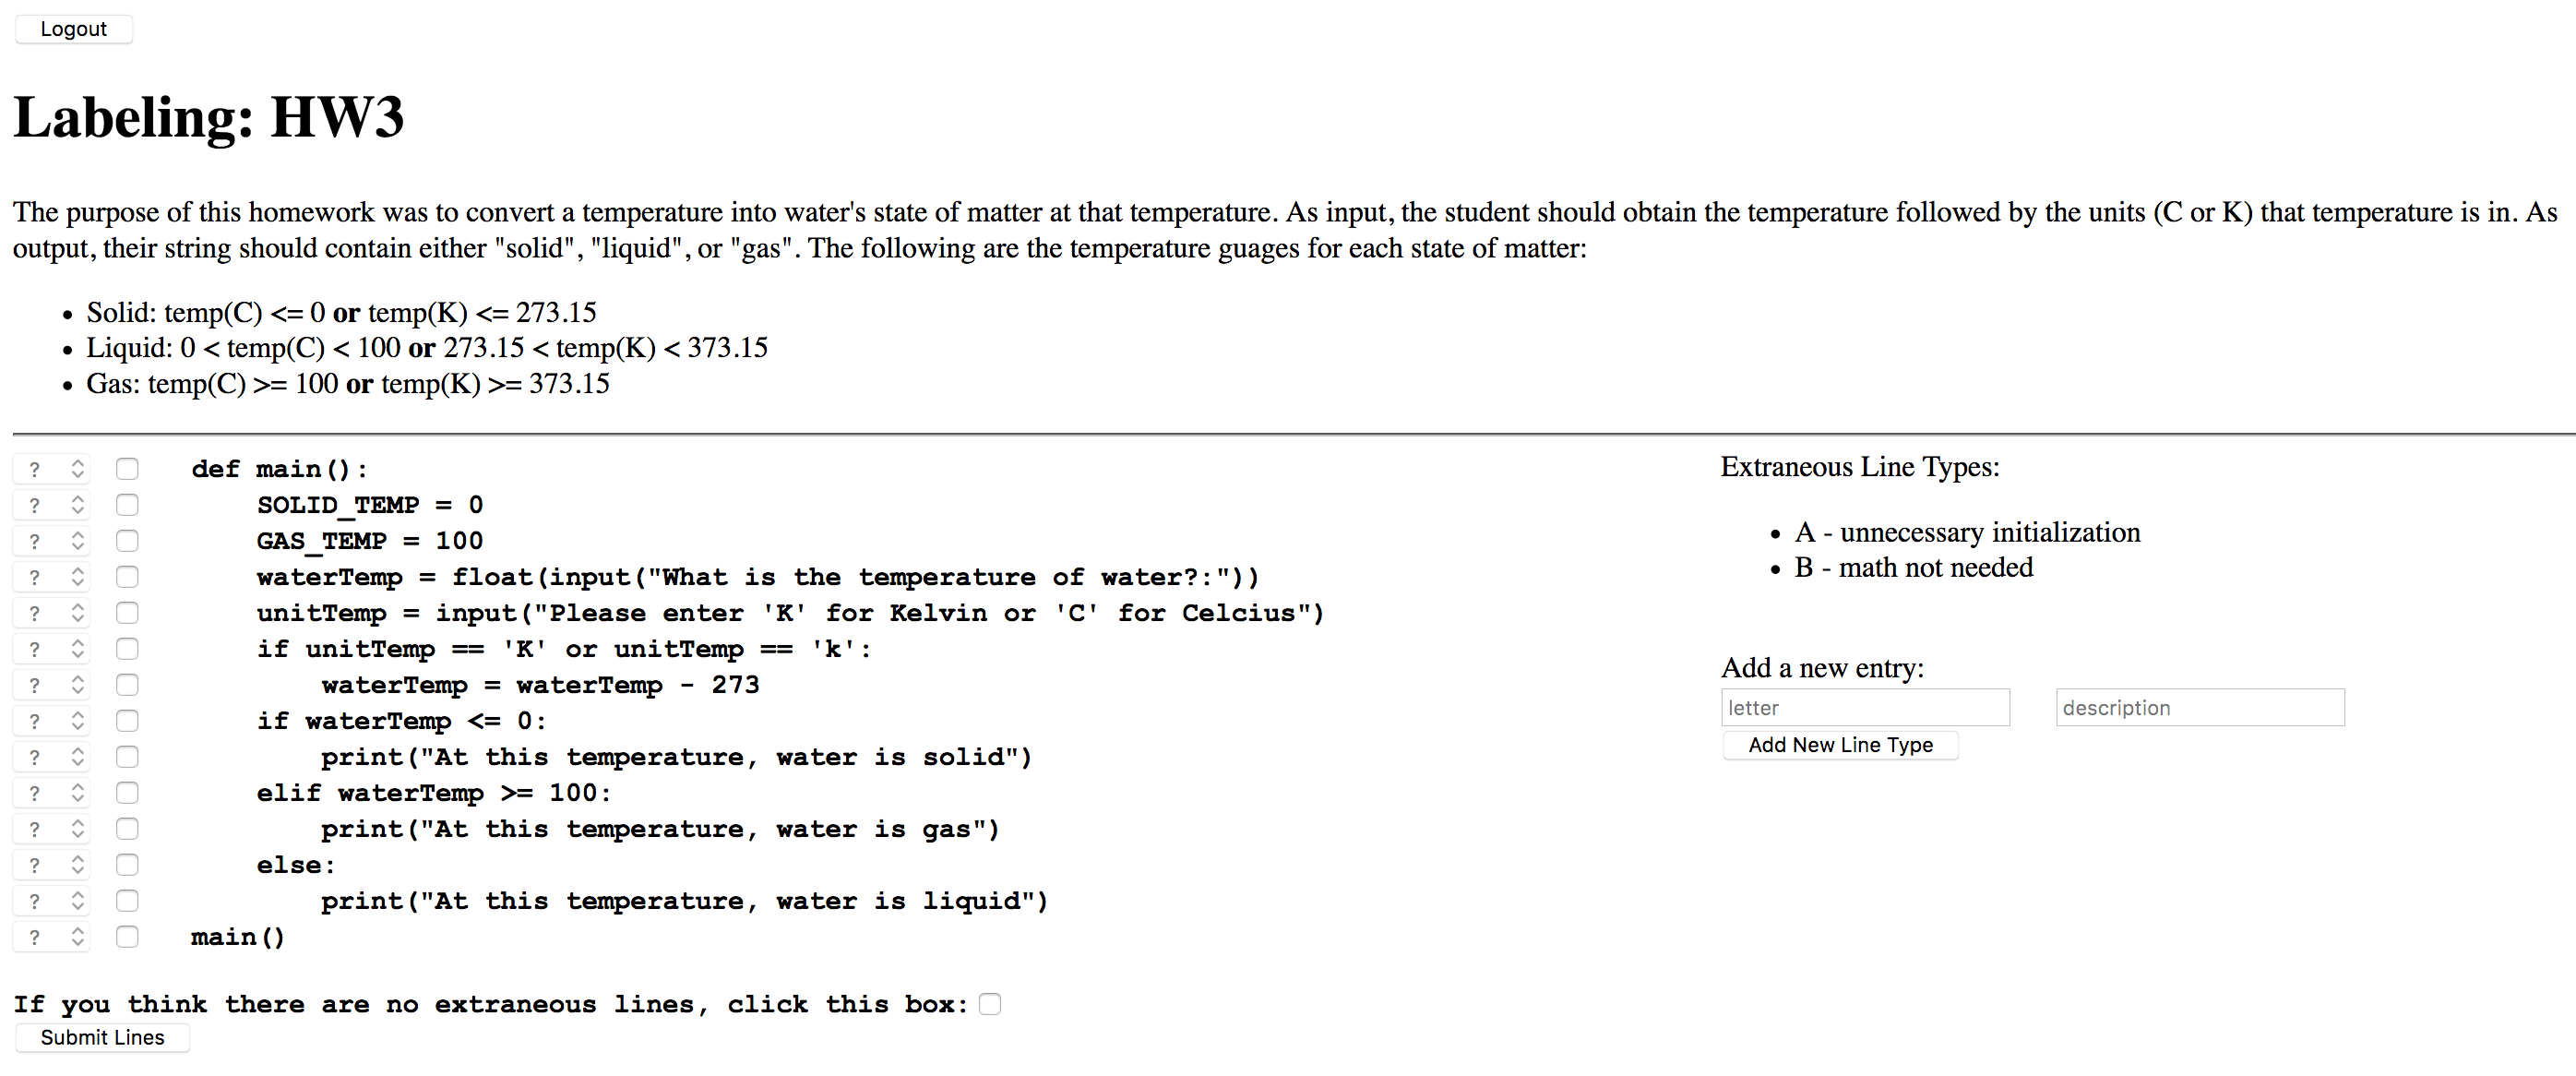
\includegraphics[width=\textwidth]{figures/webapp.png}
  \caption{Sample screen of a student labeling an assignment.}
  \label{fig:webapp}
\end{figure}

I built a custom web application to standardize the collection of labels. It allows me to easily collect different sets of labels from different people. Each user of the application reads each program, and determines which lines, if any, are extraneous. The application expedites the process of labeling, since navigating between assignments and keeping track of what has already been labeled is taken care of for the user. Figure \ref{fig:webapp} shows a sample screen for a single assignment. On the top of the page,there is a description of the problem, including any guidelines as to what constitutes a correct solution, for their reference. On the left-hand side of the screen, they can view the source code line-by-line. A line is marked as extraneous by clicking a checkbox next to the line in this area and choosing a letter from a drop-down menu. The experts were required to supply a short description of why they marked a line as extraneous. Each expert developed a unique mapping of letter to description to save time in the labeling process. On the right-hand side of the screen they can create a new mappings and view any mappings they have already made. The short description helps me to determine the reliability of each expert labeler. I can compare the lines that multiple experts marked as extraneous, and use the descriptions that the experts provide to verify whether or not that label makes sense.

% Student A - Beatriz
% Student B - Harsh
% Student C - Keith
% Student D - Zoee

\subsection{Label Reliability}

The results of each experiment are heavily influenced by the reliability of the experts who labeled the data sets. The labelers were carefully chosen such that their overall experience would better inform their selection of extraneous lines. To protect the identity of these experts I will refer to them only as Expert A, B, C, or D. Experts A and D are female, while experts B and D are male. Each expert is an undergraduate computer science major who has completed the gateway requirements, meaning that they have all passed the first three introductory courses in the computer science major (CMSC 201 - Introductory Programming in Python, CMSC 202 - Object Oriented Programming, and CMSC 341 - Data Structures). Each expert has also served as a teaching assistant for at least one of these introductory courses. In the teaching assistant position, they helped many inexperienced students with homework assignments, and were responsible for grading those assignments. Having passed the gateway for the major and held a TA position in an introductory course, these experts have experience with identifying lines of code that are not necessary to satisfy the goal of a programming assignment.

I explained to each of these four experts the definition of "extraneous lines of code" used in this work. I did so in a uniform manner as not to bias the labels produced by anyone. The experts were allowed to ask for clarification on the definition at any time, but I did not comment on any question they had regarding a specific line of code. What follows is a brief analysis of the labels produced by each of the four experts.

\vspace{2em}
\bottomcaption{Set of labels produced by Expert A.}\small
\begin{supertabular}{crrp{.5\textwidth}}
\label{labelsA}
Letter & Problem \#1 & Problem \#2 & Description \\ 
\toprule
A & 73 & 114 & unnecessary conversion of input to string \\
B & 1 & 3 & statement has no effect \\
C & 19 & 0 & conditional that has no effect \\
D & 1 & 0 & unnecessary print inside of input \\
E & 18 & 0 & statement never reached \\
F & 10 & 10 & unnecessary conversion of a variable type \\
G & 1 & 0 & unnecessary variable \\
H & 2 & 0 & while loop should've been if statement \\
I & 13 & 0 & duplicate code \\
Y & 0 & 202 & unnecessary start and/or step for range function \\
Z & 0 & 18 & loop that only executes once \\
\bottomrule
\textbf{Total:} & 138 & 347 & \\
\end{supertabular}
\vspace{2em}

Expert A produced the set of labels described in Table \ref{labelsA}. This expert labeled a total of 478 distinct lines across 295 unique files, yielding 1.62 lines per file. This expert labeled the fewest lines per file overall. The type of line that was most identified by this expert concerned an unnecessary start/stop with Python's range() function. This is a common mistake made by novice Python programmers, because there are multiple default behaviors of this function. Some of the lines identified by expert A might not actually be extraneous, such as those with label H or Z. The descriptions of these labels identify a programming construct that was used incorrectly, but that does not mean that the usage of that construct at that particular point was entirely unnecessary to solve the problem. 

\vspace{2em}
\bottomcaption{Set of labels produced by Expert B.}\small
\begin{supertabular}{crrp{.6\textwidth}}
\label{labelsB}
Letter & Problem \#1 & Problem \#2 & Description \\ 
\toprule
A & 24 & 0 & Constant not used \\
B & 19 & 0 & Extraneous conditional where one or more conditionals have no affect in execution  \\
C & 117 & 122 & Extraneous type cast \\
D & 23 & 0 & Extraneous line duplication \\
E & 86 & 26 & Unnecessary line because it is extra information that does not achieve the program's core functionality requirement \\
F & 3 & 0 & Self Assignment \\
G & 453 & 44 & Extraneous syntax \\
H & 1 & 0 & Unnecessary return \\
I & 159 & 1 & No conditional required or should be default case (i.e. elif is not required if it is the base case)  \\
J & 1 & 0 & This line assumes that water is frozen if the temperature is less than K\_BOIL, which is not true. Water is frozen if below 273 \\
L & 3 & 20 & This operation should not be required \\
M & 6 & 18 & Unnecessary declaration  \\
N & 5 & 0 & Unnecessary operation exit() because using elif will ignore following cases if a previous if statement is true \\
O & 6 & 0 & This value is always overwritten in the following control flow, and is therefore always defined when it is actually used \\
P & 0 & 1 & Range defaults from 0 to n and the 0 is not required \\
Q & 0 & 13 & Unnecessary for loop \\
R & 0 & 2 & Counter not used \\
S & 0 & 11 & The default step of range is 1 \\
T & 0 & 108 & The default start of range is 0 \\
U & 0 & 4 & This function call / declaration does not accomplish anything \\

\bottomrule
\textbf{Total:} & 906 & 370 & \\
\end{supertabular}
\vspace{2em}

Expert B produced the set of labels described in Table \ref{labelsB}. This expert labeled a total of 1276 distinct lines across 466 unique files, yielding 2.73 lines per file. This expert identified the most types of extraneous lines in the data. They were seemingly more relaxed in what they understood to be extraneous, as their most identified extraneous line type simply ``extraneous syntax." This label included lines that had unnecessary parentheses, semicolons, and a few other piece of syntactic sugar that Python understands. At the same time, they were very specific with most of their labels. The labels generated by this expert were usually more informative than the other three students, sometimes including information related to a specific problem. This expert clearly put a substantial amount of effort into the labeling process. The most interesting thing about this expert's labeling is the choice of granularity. They lumped together all extraneous syntax into one category, but split up the same general range() function mistakes into several different categories. 

\vspace{2em}
\bottomcaption{Set of labels created by Expert C}\small
\begin{supertabular}{crrp{.5\textwidth}}
\label{labelsC}
Letter & Problem \#1 & Problem \#2 & Description \\ 
\toprule
A & 71 & 37 & unnecessary print \\
B & 18 & 44 & unnecessary initialization \\
C & 66 & 0 & error-handling that does not contribute to solution \\
D & 18 & 6 & unnecessary conditional \\
E & 324 & 1 & an if/elif should be an elif/else \\
F & 71 & 111 & str() used on input() \\
G & 1 & 0 & unnecessary input \\
I & 6 & 0 & exit() not necessary \\

\bottomrule
\textbf{Total:} & 575 & 199 & \\
\end{supertabular}
\vspace{2em}

Expert C produced the set of labels described in Table \ref{labelsC}. This expert labeled 774 distinct lines across 369 unique files, yielding 2.10 lines per file. The type of line that they identified the most in the data has to due with a mistakenly used programming construct. It seems like the extraneous line marked here is a case of incorrectly applied logic, where the program author is performing an unnecessary test of a condition that could be accomplished with less code. This is a very specific extraneous line that my system may not be able to identify, as the construct is likely still necessary at that point in the solution even though there is a better way to write it that does not require that extra test. The next most identified line by this expert describe an unnecessary type cast on an input statement, similar to each of the other students. Based on their generated labels, I believe that this student has the most accurate internal definition of what it means for a line of code to be extraneous. 

\vspace{2em}
\bottomcaption{Set of labels created by Expert D}\small
\begin{supertabular}{crrp{.5\textwidth}}
\label{labelsD}
Letter & Problem \#1 & Problem \#2 & Description \\ 
\toprule
A & 2 & 0 & opportunity for compound assignment \\
B & 116 & 124 & unnecessary casting \\
C & 13 & 0 & semicolon to end line \\
D & 2 & 0 & unnecessary return \\
E & 2 & 0 & self assignment \\
F & 560 & 208 & unnecessary parenthesis \\
G & 17 & 6 & added to assignment \\
H & 4 & 0 & Debug statement \\
I & 1 & 0 & condition always true or always false \\
J & 2 & 7 & unused variable \\
K & 2 & 5 & renamed variable \\
L & 1 & 0 & print in input \\
M & 0 & 6 & Always loops once \\
N & 0 & 3 & performs no function \\
O & 0 & 7 & unnecessary initialization \\
P & 0 & 4 & unnecessary parameters \\

\bottomrule
\textbf{Total:} & 722 & 370 & \\
\end{supertabular}
\vspace{2em}


Expert D produced the set of labels described in Table \ref{labelsD}. This expert labeled 1092 distinct lines across 423 unique files, yielding 2.58 lines per file. The majority (70\%) of the lines labeled by expert D as described as having "unnecessary parentheses." Again, the majority of liens marked by this student are extraneous due to a syntax choice rather than an extraneous step in the algorithm. Some of the descriptions provided by this expert are not as informative as they could be, such as "added to assignment" or "performs no function." Upon further inspection lines with labels such as these are either just print statements that aren't directly related to the goal of the problem, or some only random statement that is unrelated to the goal. My system should, however, be able to pick up lines aptly labeled "unused variable" or "renamed variable" as these may be valid extraneous steps in the algorithm for a particular problem. It seems as though this expert made a concerted effort to be granular in their labels, but ended up with a few liens types that probably belonged lumped in the same category. 

\subsubsection{Inter-rater reliability}

Based on the labels produced, each expert clearly had a different internal definition for code that doesn't make sense in the context of a problem. Some experts took a severe approach by including any line of code with inconsequential syntax as extraneous. For example, both sets of labels created by expert B and expert D are dominated by lines of code with unnecessary syntax. Each of the four experts identified some form of unnecessary casting of variable type. There are also instances of experts having a relaxed understanding of extraneous lines of code. For example, <EXAMPLE HERE>. 

One noticeable trend in the expert labels is the identification of unnecessary syntax as an extraneous line of code. From the standpoint of the expert it is clear that lines with extra symbols that do not contribute to the overall solution to the problem should fall within the definition of extraneous line of code. Static code checking tools [CITE SOME] already exist to solve this exact problem of unnecessary syntax, and my system is not designed to report such lines. Therefore, <SHOULD I REMOVE SYNTAX RELATED LABELS?>

Another noticeable trend in the expert labels is the identification of
    

\begin{itemize}
    \item organize this section, one paragraph or so per trend, provide insight into why trend is seen, does it make sense in the context of this work?
    \item provide numbers on how many unique files and the average line count per file for each student, did one student actually label a lot more than others?
\end{itemize}

\begin{table}[htbp]
\caption{Problem 1 Breakdown}
\label{expert1}
\begin{tabular}{ll}
\textbf{Files labeled}       & \textbf{Total submissions}      \\
373                 & 466                    \\
\multicolumn{2}{l}{\textbf{Expert Agreement By Line}} \\
Single Expert       & 724                    \\
Two Experts         & 548                    \\
Three Experts       & 83                     \\
Four Experts        & 68                     \\
Total labeled       & 1423                  
\end{tabular}
\caption*{There were 1423 unique lines labels by the experts. This table shows the amount of agreement that exists between them.}
\end{table}

\begin{table}[htbp]
\caption{Problem 2 Breakdown}
\label{expert2}
\begin{tabular}{ll}
\textbf{Files labeled}       & \textbf{Total submissions}      \\
311                 & 467                    \\
\multicolumn{2}{l}{Expert Agreement By Line} \\
Single Expert       & 364                    \\
Two Experts         & 197                    \\
Three Experts       & 40                     \\
Four Experts        & 102                    \\
Total labeled       & 703                   
\end{tabular}
\caption*{There were 703 unique lines labels by the experts. This table shows the amount of agreement that exists between them.}
\end{table}

\subsection{Problem 1}
CMSC 201 received 466 unique submissions for this problem in Fall 2016. Table \ref{expert1} shows the breakdown of how those lines were labeled by the experts. 

Talk about overall trends in the expert analysis here.

\subsection{Problem 2}
CMSC 201 received 467 submissions for this problem during Fall 2016. Table \ref{expert2} shows the breakdown of how those lines were labeled by the experts.

Talk about the overall trends in the expert analysis here. 

% something similar to the below for every student?
%Although Student A identified almost twice as many unique files for this problem, the average number of lines per file is roughly the same. The culprit seems to be that Student A considers an unnecessary start and/or step in the range() function to be extraneous, as that account for more than half of the lines they identified as extraneous.

{\color{red} }

\section{Experiments}
The experiments that I carried out are the same for each problem. I ran my system eight different times on the data that I have for both problems. The ability to turn different types of dependencies on or off is built into my detection algorithm, so each run reflects one possible combination of line dependency types that are turned on. A dependency type being "turned on" means that the detection algorithm is actively using that type of dependency {\color{red}(REFERENCE PRIOR CHAPTER)} to inform its detection of lines in source code. Different permutations of line dependencies used by the system should help to visualize the impact that different dependency types have on detecting extraneous lines of code. Some combinations of extraneous line type will likely offer no insight in this regard. The case where all three dependency types are turned off in the detection algorithm will be ignored in this section as a result, but the relevant data is provided in {\color{red} (SHOULD AN APPENDIX GO HERE?)}

% paragraph about experimentation set up, and logging


Experimentation with my system is limited by the correctness of each target program. My system is entirely dependent on the completeness and correctness of the target program is it analyzing. For each problem, there are specific student solutions that contain errors. These programs are left out of the following analysis. If the program that I run through my system contains any sort of errors, due to incorrect syntax or otherwise, then I cannot detect extraneous lines in that program. This is a consequence of the dependence on matching the goal output. If a program breaks for any reason, there will not be any output lines that mach the goals of that particular problem. 

In order to test the accuracy of my system, I must compare what it views as extraneous to what the experts view as extraneous. The experts labeled a significant number of individual lines, but to get more of sense of the accuracy and precision of this system I will only focus on the lines of code where there was a consensus by the experts. The relevant data is available in appendix {\color{red}(AGAIN, SHOULD THERE BE AN APPENDIX OF DATA?)}. I define expert consensus as a line of code where a majority of the experts agree on its extraneous status. A line labeled by three or four experts constitutes a majority. I believe that a line of code that has been labeled by the experts in the same manner is more likely to actually be what the experts claim it is, therefore it is more likely that my system will pick up on that same line. 

{\color{red} \textbf{ do I need a summary paragraph here?}}

\subsection{Problem 1}

The first problem that my system as


\begin{table}[htbp]
\caption{The errors detected in Problem 1}
\begin{tabular}{ll}
Failure      & Amount \\
GoalNotFound & 90     \\
TraceError   & 23     \\
SyntaxError  & 8     
\end{tabular}
\end{table}

% each of the following items in this list are one experimentation method that I will include. I need to rerun a few of these results, and figure out some numbers before I write this up. Do I need to include all 7 permutations in my analysis, or should I justify not showing all of them somehow? Also, I need to figure out a better way of graphically representing the information 

% no you dont include all 8

%\subsubsection{Analysis}
%This is where I talk about specific intuitions regarding the first problem.

%\subsection{Problem 2}
%This is where I describe the setup for the second problem.

%\subsubsection{Analysis}
%This is where I talk about specific intuitions regarding the second problem.

%\section{Conclusion}
%Remaining items to discuss:
%\begin{itemize}
%    \item number of files and lines labeled by each student
%    \item overall trends in the labels (any other than type casting and syntax?)
%    \item show experiment results with HW3 and HW5 (HW3 experiments complete, need to tweak HW5 slightly)
%    \item explain what experiments matter
%    \item how did the system do compared to experts?
%    \item label my own data for a baseline 
%\end{itemize}



\end{document}
